
\section{Eigenschaften des Verhandlungsführers}


\begin{frame}{Table of contents}
  \setbeamertemplate{section in toc}[sections numbered]
  \tableofcontents
\end{frame}

\subsection{Einfühlungsvermögen}

\begin{frame}
  \begin{framed}
    \textquote[\cite{obermeier_karrieresprung_nodate}]{Steige nie mit rationalen Argumenten ein.} 
  \end{framed}
\end{frame}


\begin{frame}{Forderungen und Bedürfnisse}

  \begin{columns}[c]
    \begin{column}{.55\textwidth}

      {\small
      \begin{itemize}
        \item Motive, Bedürfnisse hinter den Forderungen des Gegenübers verstehen
          \cites[][p. 106]{mccarthy_advanced_2015}[][p. 156]{wannenwetsch_schluesselfaktoren_2009}
        \item Analysieren \cite[][ch. 4.4.2]{helmold_verhandlungskonzepte_2019}
          {\footnotesize
          \begin{itemize}
            \item Primärmotive: lebensnotwendig,\\z.B. Hunger, Geborgenheit
            \item Sekundärmotive: angelernt,\\z.B. Anerkennung, Erfolg
          \end{itemize}
          }
        \item Irrationalität im Verhalten \cite[][p. 12]{mccarthy_advanced_2015}
        \item Sachliche Argumente können unbedeutend werden 
      \end{itemize}
      }

    \end{column}

    \begin{column}{.35\textwidth}
      
\includegraphics[width=\textwidth]{content/fig/eisberg.jpg}
      {\hspace*{15pt}\hbox{\scriptsize\itshape Credit:\thinspace{\cite{eisberg_fig}}}}
    \end{column}
  \end{columns}

\end{frame}

\begin{frame}{Empathie vs. Hineinversetzen}

  \begin{block}{Hineinversetzen}
    \enquote{Es gibt immer zwei Seiten der Medaille und ich versuche beide zu sehen.}
  \end{block}
  \begin{block}{Empathie}
    \enquote{Manchmal tut es mir gar nicht so leid, wenn es Leuten schlecht geht.}
  \end{block}

  Das Hineinversetzen ermöglicht effizientere Abmachungen mit größerem kollektiven und individuellen Zugewinn \cite{galinsky_why_2008}.

  Was helfen kann: Behavioristische Mimikry \cite[][p. 500]{thompson_negotiation_2010}
\end{frame}

\note[itemize]{
  \item can be applicable in certain negoations:
  \item angry negotatiors with desire to be heard
  \item calming, softening, de-escalation
  \item helpful in mediation
}

  

\begin{frame}{\enquote{Der erste Eindruck zählt}}
  Mentales Modell: kognitive Repräsentation der erwarteten Verhandlung \cite[][p. 287ff]{bazerman_negotiation_2000}
  \begin{itemize}
	\item Beziehungen
	\item Attributionen
	\item Struktur und Prozess
  \end{itemize}

  Individuelle Mentale Modelle können zu Beginn einer Verhandlung häufig Feindlichkeit erwarten.
  Erst über den Lauf der Verhandlung wird über Win-Win-Potenziale gelernt. Wenn sich die Wahrnehmung ändert, dann nur sehr früh zu Beginn \cite{thompson_social_1990}
    \cite[][p. 287ff]{bazerman_negotiation_2000}. 

\end{frame}

\note[itemize]{
  \item konstante Musterkennung
  \item Zuordnung zu einer Schublade, zu Rollen (Geschäftspartner, Freund) 
  \item ohne Verbindung zur Realität
}


\begin{frame}{Persönlichkeitstypen}
  \begin{columns}[c]
    \begin{column}{.55\textwidth}
     Der Eigene wie auch der des Gegenüber sollte eigenschätzt werden
        \cite[][ch. 4.5.5]{helmold_verhandlungskonzepte_2019}.

      Myers-Briggs-Typenindikator:
      \begin{itemize}
        \item \textit{Sensing-Thinking}: klare Fakten, gute Argumente
        \item \textit{Intuition-Feeling}: Vertrauen aufbauen, Respekt ausstrahlen
      \end{itemize}
    \end{column}
    \begin{column}{.35\textwidth}
      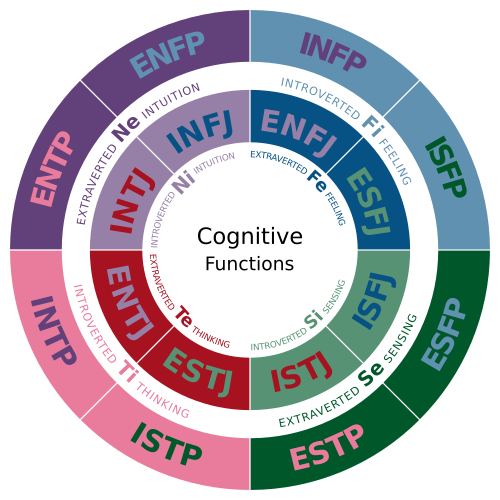
\includegraphics[width=\textwidth]{content/fig/mbti.png}
      {\hspace*{15pt}\hbox{\scriptsize\itshape Credit:\thinspace{\cite{mbti_fig}}}}
    \end{column}

\end{columns}


    
\end{frame}


\subsection{Respekt}

\begin{frame}{Respekt \ldots}

  \begin{itemize}
    \item[\ldots] gegenüber dem Verhandlungspartner: Grenzen kennen
    \item[\ldots] gegenüber sich selbst: Selbstbewusstsein
    \item[\ldots] ausstrahlen: Körpersprache
  \end{itemize}

\end{frame}

\begin{frame}{Respekt zollen}

  \begin{itemize}
    \item Zuerst eine Beziehung aufbauen, dann Fakten schaffen \cite[][p. 16]{mccarthy_advanced_2015}
    \item Vertrauen schaffen, um mentale Hürden zu senken und den Informationsaustausch zu fördern \note{-> Integrativ}
    \item Aufmerksames, aktives Zuhören (siehe \hyperref[sec:geduld]{Geduld})
    \item Notizen nehmen \note{Erinnerungen, Aufmerksamkeit zeigen}
  \end{itemize}

\end{frame}

\begin{frame}{Selbstbewusstsein}

  % TODO Raus schmeißen?
  Propriozeptive Psychologie: \enquote{Fake it `til you make it} \cite[][p. 38]{mccarthy_advanced_2015}

  \note{Experiment: Leute for dem Computer bildschirm – horizontal und vertikal bewegende Teile}
  \note{people smile when they're happy, but they're also happier because they smile}

  Kann also indirekt gewonnen werden über \ldots 

\end{frame}

\begin{frame}{Ausstrahlung}

  \begin{columns}[c]
    \begin{column}{0.55\textwidth}
      {\small

      Kongruentes Verhalten ist glaubwürdig: Körper, Stimme und Inhalt müssen sich decken \cite[][p. 161ff]{wannenwetsch_schluesselfaktoren_2009}.

      93\% der Wirkung sind unabhängig vom Inhalt \cite[][p. 164]{wannenwetsch_schluesselfaktoren_2009}.

      \note{können auch negative Ausdrücke sien: bei unrealistischen Forderungen}

        Säulen:
        \begin{itemize}
          \setlength\itemsep{0em}
          \item Mimik und Gestik \note{kann schwer festgemacht werden}
          \item Körperhaltung
          \item Blickkontakt \note{kein Starren}
          \item Kleidung: ordentlich, sauber, dezent, passend \note{auch zur Persönlihckeit}
          \item Stimme: Verständlichkeit und Modulation \note{Spannung erzeugen, Positionen, Prioritäten hervorheben, aber keine Lautstärke = Dominanz}
        \end{itemize}
      }
    \end{column}
    \begin{column}{0.35\textwidth}
      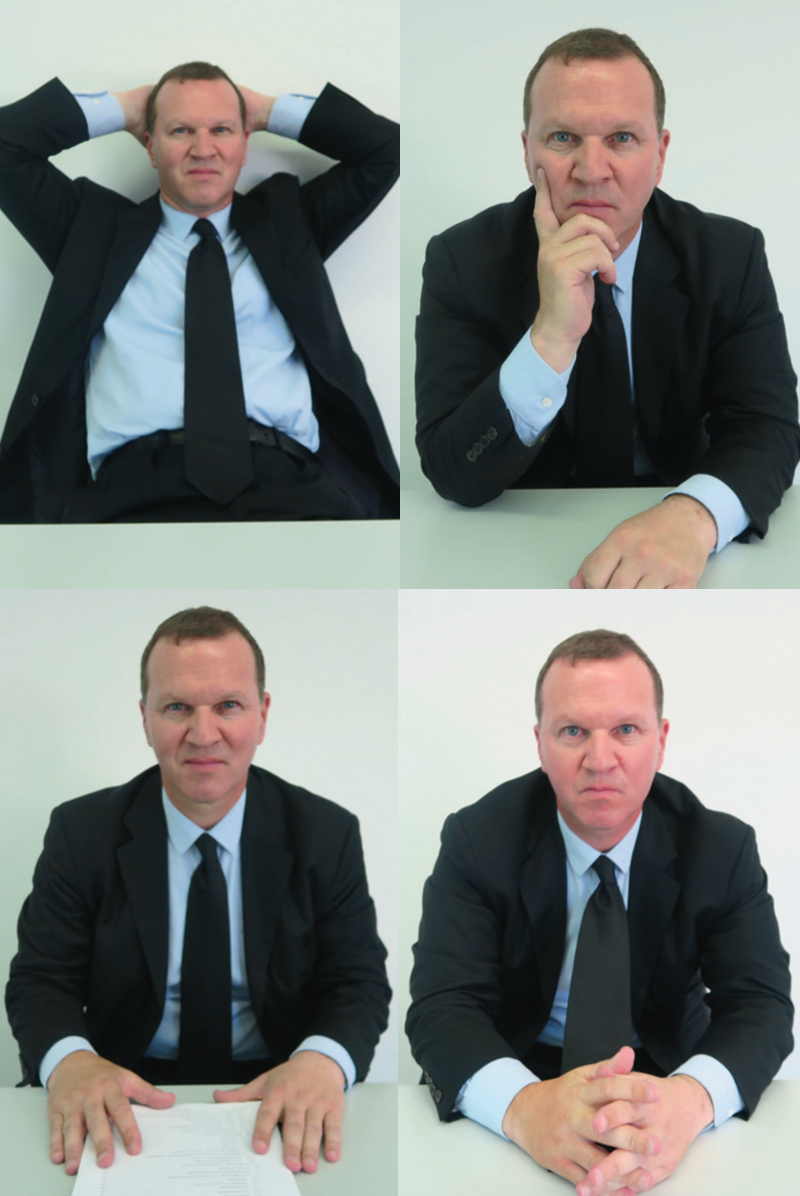
\includegraphics[width=\textwidth]{content/fig/nonverbal.png}
      {\hspace*{15pt}\hbox{\scriptsize\itshape Credit:\thinspace{\cite{helmold_nonverbale_2019}}}}
    \end{column}
  \end{columns}

\end{frame}


\subsection{Integrität}

\begin{frame}{Täuschungen\ldots}

  \begin{itemize}
    \item[\ldots]passieren häufiger, wenn mehr auf dem Spiel steht \cites[][p. 292]{bazerman_negotiation_2000}[][p. 501]{thompson_negotiation_2010}
    \item[\ldots]zerstört Vertrauen und verringert damit die Chancen auf integrative Lösungen % TODO definition
    \item[\ldots]kommt von einer Kombination aus Versuchung, Unsicherheit, Machtmangel und Anonymität von Opfern \cite[][p. 501]{thompson_negotiation_2010}
  \end{itemize}

\end{frame}

\begin{frame}{Integrität}
  Gesellschaftiche Regeln sollten eingehalten werden:

  \begin{itemize}
    \item Ehrlichkeit
    \item Zuverlässigkeit
    \item Pünktlichkeit
    \item Legalität
    \item keine Machtinstrumentalisierung
    \item Fairness
    \item Verantwortungsbewusstsein \note{Entschludigung, Formalitäten, Dokumente, Termine}
  \end{itemize}

  Freunde mit kommunaler Orientierung sind am wahrscheinlichsten dazu in der Lage beidseitige Zugewinne zu sichern \cite[][p. 502]{thompson_negotiation_2010}.
  \note{ohne Erwartungen auf Rückzahlung <-> kommunale Orientierung: Austausch-Orientierung, aufhebende Gegenseitigkeit von wohlwollenden Handlungen}
  
  Pragmatisch sein: persönliche Emotionen wahrnehmen, aber nicht immer zeigen. Sie können einen negativen Effekt auf Verhandlungen haben. \cite[][p. 13]{mccarthy_advanced_2015}
\end{frame}

\begin{frame}{Fairness}

  Eine Definition kann vom Kulturkreis und der Vergangenheit abhängen \cite{rabin_incorporating_1993}. \note{vergangener Preis}
  
  Altruismus motiviert Altruismus, Hass befördert Hass. Für beides sind Menschen bereit Materielles aufzugeben. Je niedriger die materiellen Kosten, desto größer diese Effekte. \cite{rabin_incorporating_1993}

  Wünsche und Bedürfnisse aller sollten berücksichtigt werden. Doch \textquote[\cite{obermeier_karrieresprung_nodate}]{es geht nicht um reale, sondern gefühlsmäßige Win-Win Situationen.} 

\end{frame}

\subsection{Geduld} \label{sec:geduld}

\begin{frame}
    
  \begin{columns}[c]

  \begin{column}{0.55\textwidth}

    Positives Denken \cite[][p. 33ff]{mccarthy_advanced_2015}
    \begin{itemize}
      \item die Einstellung bestimmt das Verhalten
      \item Konflikte als Möglichkeit, statt Problem
      \item inhärentes Vertrauen
      \item schafft Motivation und Geduld
    \end{itemize}
  
    Zweite Versuche sind meist notwendig und Teil des Wegs zum Erfolg. 

  \end{column}
  
  \begin{column}{0.35\textwidth}
      
\includegraphics[width=\textwidth]{content/fig/brickwall.jpg}
      {\hspace*{15pt}\hbox{\scriptsize\itshape Credit:\thinspace{\cite{brickwall_fig}}}}
  \end{column}


\end{columns}

\end{frame}

\begin{frame}

  Eine Form Geduld zu zeigen: Aktives Zuhören
  
  \begin{itemize}
    \item animiert zum Weiterreden
    \item ist konzentriertes, eingehendes Zuhören
    \item beinhaltet Feedback und Verständnis-Fragen: Johari-Fenster \cite[][p. 97]{mccarthy_advanced_2015} \note{gegenseitig Blind Spots entfernen}
    \item beachtet auch Betonung und Körpersprache
    \item zollt Respekt
  \end{itemize}
    
  \enquote{Schweigen ist Gold}. Nach überzeugenden Argumenten und wenn man nichts zu sagen hat sollte man schweigen \cites{obermeier_karrieresprung_nodate}[][ch. 4.5.2]{helmold_verhandlungskonzepte_2019}.

\end{frame}


\subsection{Humor und Kreativität}

\begin{frame}
  \begin{block}{Humor}
    Die Fähigkeit auch in schwierigen Situationen Amüsantes zu erkennen.
  \end{block}

  Humor hilft der Kreativität. Diese besteht aus Spontanität, Phantasie und Originalität und schafft Handlungsspielräume und damit Möglichkeiten zur Einigung 
   \cite[][p. 159]{wannenwetsch_schluesselfaktoren_2009}.

\end{frame}

\begin{frame}

  Mentale Vorbereitung kann helfen \cite[][p. 169f]{wannenwetsch_schluesselfaktoren_2009}

  \begin{itemize}
    \item Propriozeptive Psychologie \cite[][p. 37ff]{mccarthy_advanced_2015}
    \item Befreiung von Zwängen
    \item Einstellung: Interesse, Neugier oder Langeweile, Desinteresse?
  \end{itemize}

\end{frame}


\subsection{Selbstdisziplin und Durchhaltevermögen}

\begin{frame}{Selbstdisziplin}

  Eigen-Motivation, Autarkie, Selbstbestimmtheit

  kann gefördert werden durch\ldots
  \begin{itemize}
    \item[\ldots]Fokus auf Stärken, statt Schwächen \note{mehr Spaß, inhärenter Antrieb}
    \item[\ldots]Kontrolle über Emotionen: Zorn und Begeisterung ggü. Offenheit und Interesse
    \item[\ldots]Vorstellung vom Erfolg \note{am Strand}
    \item[\ldots]Zelebrieren des Erfolgs \note{feiern!}
  \end{itemize}

  \ldots und fördert das Durchhältvermögen\ldots

\end{frame}

\begin{frame}{Durchhaltevermögen}

Ohne guten Grund nachzugeben kann Misstrauen fördern. Es sollten nur dann Zugeständnisse gemacht werden, wo sie von Nutzen sind (Gegenleistungen). \cites{obermeier_karrieresprung_nodate}[ch. 4.5.2]{helmold_verhandlungskonzepte_2019}.

  Es sollte stets versucht werden, die Argumente der Gegenseite zu entkräftigen. Man darf nach Evidenz verlangen. Der Fokus sollte auf den schwächsten Argumenten der Gegenseite liegen \cite[][ch. 4.5.2]{helmold_verhandlungskonzepte_2019}.

\end{frame}

\begin{frame}

  \ldots und alles baut auf dem Fundament:
  
  Gesunde Ernährung, Schlaf und Work-Life Balance.

\end{frame}

